% LaTeX file for a 1 page document
\documentclass[10pt]{article}

\usepackage{fancyvrb}
\usepackage{graphicx}
\usepackage{verbatim}
\usepackage[italian]{babel}
\usepackage{mathtools}
\usepackage{multirow}
\usepackage[utf8]{inputenc}
\usepackage{amssymb}


% Pdf utilities
\usepackage[pdftex,bookmarks,colorlinks,%
pdfauthor={Daniele Bellavista},%
pdftitle={Framework per la simulazione e la valutazione di modelli CTMC
utilizzando Maude e Approximate Probabilistic Model Checking},%
pdftex]{hyperref}
\hypersetup{colorlinks=false}

\title{Framework per la simulazione e la valutazione di modelli CTMC
utilizzando Maude e Approximate Probabilistic Model Checking}

\author{Bellavista Daniele}

\begin{document}
\maketitle

\section{Introduzione}

Nella prima parte di questo progetto ho implementato un simulatore per modelli
CTMC (\emph{Continuos time Markov Chain}) generici, cioè senza assunzione sulla
struttura degli stati del sistema. Questo obiettivo è stato raggiunto in
primis utilizzando Maude e il matching simbolico nativo, ma anche
grazie all'utilizzo del meta-livello di Maude \cite{maudemanual}, che permette
di trasformare moduli Maude in dati e di eseguire operazioni dinamiche su di essi.

Nella seconda parte, ho implementato un verificatore di proprietà
PCTL monotone utilizzando la tecnica di \emph{Approximate Probabilistic Model
Checking} \cite{DBLP:conf/vmcai/2004}\cite{HLMP04}.

\section{Il meta-livello di Maude}

La logica di \emph{rewriting} di \emph{Maude} è riflessiva \cite{maudemanual},
ovvero descritta in termini di se stessa tramite una teoria universale. 
Rendendo disponibile all'utente l'accesso alla teoria universale di Maude, è
possibile ragionare ponendosi al meta-livello sia della \emph{``struttura''} dei
moduli e termini \emph{Maude}, sia delle strategie risolutive dei procedimenti
di inferenza, riduzioni, matching e ricerche.

La \emph{riflessione} della logica di rewriting può essere descritta attraverso
la relazione :

\[
	\mathcal{R} \vdash t \to t' \Leftrightarrow \mathcal{U} \vdash \langle
	\bar{\mathcal{R}}, \bar{t} \rangle \to \langle \bar{\mathcal{R}'},	\bar{t'}
	\rangle
\]

Dove $\mathcal{R}$ è una teoria di \emph{rewrite},  $\mathcal{U}$ è la teoria
di rewrite universale, in grado di rappresentare qualunque teoria di rewrite
finita in termini di se stessa. Il simbolo $\to$ indica che il termine a
sinistra può essere riscritto come il termine di destra; $t, t'$ sono termini,
$\langle \bar{\mathcal{R}}, \bar{t} \rangle$ è un termine che rappresenta
secondo la teoria $\mathcal{U}$ la coppia $(\mathcal{R}, t)$.

La teoria $\mathcal{U}$ è universale e può essere espressa anche in termini di
se stessa. Dunque la relazione precedente crea una ``reflective tower'' nella
quale è possibile muoversi sia alto che in basso. Il livello più basso nella
torre è chiamato forma canonica.

La teoria universale di rewrite $\mathcal{U}$ è implementata in
Maude nel modulo \texttt{META-LEVEL}, il quale, oltre a contenere operazioni
per muoversi lungo la reflective tower, contiene sort per descrivere al
meta-livello moduli e termini.

La maggior parte delle operazioni del meta-livello di Maude
sono parziali, poiché possono esistere argomenti del Sort corretto che tuttavia
non sono una corretta meta-rappresentazione o non esiste una valido risultato.

\subsection{Accesso dinamico a moduli e termini}

Termini e moduli Maude possono essere rappresentati come altri termini Maude,
sruttando la teoria di rewriting universale, permettendo di caricare moduli
dinamicamente, lavorare e costruire termini di Sort anche sconosciuti ed
eseguire su tali meta-moduli e meta-termini delle operazioni di reduce e rewrite.

\subsubsection{upTerm e downTerm}

Dato un qualunque termine Maude, è possibile salire e scendere la
\emph{reflectio tower} utilizzando le operazioni \emph{upTerm} e
\emph{downTerm}:
\begin{Verbatim}[fontsize=\small]
op upTerm : Universal -> Term [poly (1) special (...)] .
op downTerm : Term Universal -> Universal [poly (2 0) special (...)] .
\end{Verbatim}
\emph{upTerm} prende in ingresso un qualunque termine $t$ e restituisce sempre
la sua meta-rappresentazione $\bar{t}$ di sort \emph{Term}. \emph{downTerm}
prende in ingresso $\bar{t}$, meta-rappresentazione di un termine $t$, ed un secondo argomento di
un certo kind. Se $t$ è dello stesso kind del secondo argomento, la
\emph{downTerm} restituisce $t$, altrimenti restituisce il secondo argomento.
\begin{Verbatim}[fontsize=\small]
Maude> red in META-LEVEL : upTerm ( 'a ) .
result Constant: ''a.Sort

Maude> red in META-LEVEL : upTerm( 'a 'b ) .
result GroundTerm: '__[''a.Sort,''b.Sort]

Maude> red in META-LEVEL : downTerm ( ''a.Sort , ('prova).Qid ) .
result Sort: 'a

Maude> red in META-LEVEL : downTerm ( ''a.Sort , ("Fail").String ) .
result String: "Fail"
\end{Verbatim}

\subsubsection{upModule}
\label{sec:upMod}
I comandi \emph{mod} e \emph{fmod} permettono di definire moduli che Maude
caricherà nel proprio database interno. Quando si eseguono istruzioni come
\begin{Verbatim}[fontsize=\small]
Maude> reduce in MIO-MODULO : prova( 1 , 2 , 3 ) .
\end{Verbatim}
Maude accede al database, cerca il modulo \emph{MIO-MODULO} ed effettua la
\emph{reduce} dell'espressione \emph{prova(1,2,3)}: l'accesso al database è
statico.

Il meta-livello di Maude permette di ottenere la meta-rappresentazione di un
modulo precaricato nel database, partendo dal suo nome espresso con un quoted
identifier, tramite l'operazione:
\begin{Verbatim}[fontsize=\small]
op upModule : Qid Bool ~> Module [special (...)] .
\end{Verbatim}
Il primo argomento è il nome del modulo, il secondo argomento è true se si
desidera ottenere anche la meta-rappresentazione di tutte le operazioni
derivate dai moduli importati, false altrimenti. Il valore di ritorno Module è
un particolare sort che meta-rappresenta un modulo Maude; ha una struttura
definita, con un ordine preciso, dunque è semplice da analizzare ed alterare, ma
non è possibile caricare un meta-modulo nel database di Maude.

\subsubsection{metaRewrite e metaApply}
\label{sec:mapply}
Dato un oggetto di tipo Module è possibile eseguire dinamicamente operazioni
di reduce, rewrite e apply (applicazione di una rule data una regola) partendo
dalla meta-rappresentazione del termine da ridurre o riscrivere. L'operazione
\emph{metaRewrite} permette di eseguire su un meta-modulo \emph{Module} la
rewrite di un meta-termine \emph{Term} fino ad un numero di volte specificato da
\emph{Bound}.
\begin{Verbatim}[fontsize=\small]
sort Bound .
subsort Nat < Bound .
op unbounded :-> Bound [ctor] .
op metaRewrite : Module Term Bound ~> ResultPair [special (...)] .
\end{Verbatim}
La metaRewrite ritorna valore di sort ResultPair:
\begin{Verbatim}[fontsize=\small]
sort ResultPair .
op {_,_} : Term Type -> ResultPair [ctor] .

op getTerm : ResultPair -> Term .
op getType : ResultPair -> Type .
\end{Verbatim}
contenente la meta-rappresentazione del risultato e la meta-rappresentazione del
suo kind o sort. La funzione \emph{metaRewrite} è parziale, quindi se Module o
Term sono sintatticamente corretti, ma non sono corrette meta-rappresentazioni,
è restituito un risultato indefinito di kind [ResultPair] .

L'operazione \emph{metaApply} (e la sua generalizzazione \emph{metaXapply})
permettono di applicare una rule basandosi sulla label ed ottenere un risultato dettagliato sulla
riscrittura. La chiamata di $metaXapply(\bar{\mathcal{R}}, \bar{t}, \bar{l},
\sigma, n, b, m)$ riduce $t$ con le equazioni di $\mathcal{R}$, dopodiché crea
una sequenza di soluzioni applicando tutte le rule chiamate $l$ al termine $t$ e
scarta i primi $n$ risultati. $b$ e $m$ specificano il livello di nesting al
quale applicare la riscrittura (per una riscrittura non limitata: 0 -
$unbounded$).
\begin{Verbatim}[fontsize=\small]
sorts Result4Tuple Result4Tuple? .
subsort Result4Tuple < Result4Tuple? .
op {_,_,_,_} : Term Type Substitution Context -> Result4Tuple [ctor] .
op failure : -> Result4Tuple? [ctor] .

op metaXapply : Module Term Qid Substitution Nat Bound Nat ~>
                                                      Result4Tuple? .
\end{Verbatim}
Se l'operazione è andata a buon fine, il risultato \emph{Result4Tuple} contiene:
\begin{description}
  \item[Term:]meta-termine riscritto.
  \item[Type:]meta-tipo del termine riscritto.
  \item[Substitution:]dettagli sulla sostituzione effettuata dalla apply.
  \item[Context:]contesto nel quale è avvenuta la riscrittura. Contiene una
  lista di meta-termini non riscritti e un singolo ``hole'' dove è avvenuta la
  riscrittura.
\end{description}

\subsubsection{metaMatch}
Un'altra potente applicazione del meta-livello di Maude è la metaMatch (e la
sua generalizzazione metaXmatch), che permette di eseguire un match fra due
meta-termini all'interno di un meta-modulo permettendo di specificare condizioni
booleane e di enumerare le soluzioni.
\begin{Verbatim}[fontsize=\small]
sorts MatchPair MatchPair? .
subsort MatchPair < MatchPair? .
op {_,_} : Substitution Context -> MatchPair [ctor] .
op noMatch : -> MatchPair? [ctor] .
op metaXmatch : Module Term Term Condition Nat Bound Nat ~>
                                             MatchPair? [special (...)] .
\end{Verbatim}
Il risultato \emph{MatchPair} contiene le sostituzioni effettuate e il contesto
nel quale è avvenuta la sostituzione.

\section{Progetto CTMC}

La prima parte del progetto che ho realizzato è un simulatore per modelli
CTMC utilizzando il linguaggio Maude e le sue funzionalità di meta-livello.

\subsection{Requisiti}
\label{sec:requisiti}

Si vuole realizzare un simulatore per catene di Markov tempo continue in grado
di:
\begin{itemize}
  \item Gestire stati arbitrari.
  \item Gestire azioni di transizione da uno stato all'altro caratterizzate da
  un certo rate, permettendo di specificare condizioni e rate dinamici.
  \item Gestire delle overview, ovvero risultati parziali dell'esecuzione.
\end{itemize}

\subsection{Realizzazione}

Una transizione è descrivibile come $State \Longrightarrow [Rate] State$ $if$
 $Condition$, ovvero come stati che possono essere trasformati in altri stati
secondo un certo rate e se è avverata una data condizione. Questa definizione è
naturalmente riconducibile alle \emph{rewriting rule} di Maude; dunque, definita
una sintassi per i membri delle rule, si può sfruttare il meccanismo di rewrite
nativo.

L'ultimo punto dei requisiti riguarda la gestione delle overview. Definisco una
Overview come una informazione che l'utente riceve ogni $M$ passi di
simulazione, contenente informazioni relative alla dinamica del sistema.

\subsection{Organizzazione}

Il sistema è suddiviso in due moduli. \emph{CTMC} contiene per la sintassi
di CTMC, che i moduli utente devono importare, mentre \emph{CTMC-ENGINE}
contiene le operazioni necessarie per la simulazione.

\subsubsection{Modulo CTMC}

All'interno del modulo \emph{CTMC} ho definito i Sort e i costruttori del
modello CTMC. Una catena di Markov è una coppia $\langle A , \rightarrow A
\rangle$, dove $A$ è un insieme di stati e $\rightarrow \subseteq A \times
\mathbb{R}_{0}^{+} \times A$ è una transizione fra due stati che avviene con un
certo rate. Come detto precedentemente, è possibile sfruttare il meta-livello di
Maude per gestire le transizioni come \emph{rule} e definire unicamente la sintassi.

Per avere una definizione più generica possibile di stato del sistema, definisco
uno \emph{State} come un elemento polimorfico:
\begin{Verbatim}[fontsize=\small]
sort State  .
op <_> : Universal -> State [ ctor poly (1) ] .
\end{Verbatim}

Per modellare i rate, ho definito un sort che comprenda rate e stato finale e
che possa essere riscritto dallo stato inziale: \emph{Config} subsort di
\emph{State}. In questo modo \emph{State} può essere riscritto come un
\emph{Config}.
\begin{Verbatim}[fontsize=\small]
sort Config Rate Var .
subsort Float < Rate .
subsort Config < State .
op [_]_ : Rate State -> Config [ ctor prec 80 ] .
\end{Verbatim}
Per semplificare ed ottimizzare le operazioni di simulazione, impongo che il
modulo utente debba definire le regole di rewrite del modello con la
label \emph{model}. Ad esempio:
\begin{Verbatim}[fontsize=\small]
*** Esempio di modello CTMC in cui lo stato è un multi-set
*** di numeri naturali. Le regole che formano il modello devono
*** avere la label model.

sort NatMSet .
subsort Nat < NatMSet .
op nil : -> NatMSet .
op __ : NatMSet NatMSet -> NatMSet [ ctor comm assoc id: nil ] .

crl [model] : < 12 N:Nat 123 > =>
                   [0.2 * float(N:Nat)] < 1312 > if N:Nat > 14 .
crl [model] : < N:Nat > =>
                   [0.8 * float(N:Nat)] < 12 15 123 > if N:Nat > 1300 .
rl [model] : < N:Nat NL:NatList > =>
                   [12.0] < (N:Nat + 1) NL:NatList > .
\end{Verbatim} 

Nel modulo \emph{CTMC} ho anche definito la sintassi per l'overview,
implementato come contenitore di una lista di \emph{Entry}, coppie
$(Tempo, Stato)$:
\begin{Verbatim}[fontsize=\small]
sort Overview Entry EntryList .
subsort Entry < EntryList .

op _:_ : Float State -> Entry [ ctor prec 80 ] .
op empty : -> EntryList [ ctor ] .
op _ - _ : EntryList EntryList -> EntryList [ ctor assoc id: empty prec 90 ] .
op [_] : EntryList -> Overview [ ctor ] .
\end{Verbatim}

Per i motivi che spiegherò in seguito, il modulo utente per la gestione
dell'overview, deve implementare un sistema di rule per riscrivere l'Overview,
tenendo conto che sarà effettuata un'unica rewrite . Per iterare l'overview si
possono comunque usare sistemi di equazioni, poiché il risultato è sempre
ridotto.

\subsubsection{Modulo CTMC-ENGINE}
\label{sec:CTMC-ENGINE}

Il modulo engine è il simulatore dei modelli CTMC. Ho realizzato questo engine
in modo che potesse simulare dinamicamente un modello, ricevendo il nome del
modulo che lo implementa e la meta-rappresentazione dello stato iniziale. In
questo modo non ha bisogno di conoscere operazioni ed sort del modulo
utente.

Utilizzando l'operazione \emph{upModule}, descritta nella sezione
\ref{sec:upMod}, il simulatore è in grado di ottenere il meta-modulo e
cominciare la simulazione eseguendo ricorsivamente una sequenza di passi:

\begin{enumerate}
  \item Trovare tutte le azioni concorrenti che possono attivarsi dallo stato
  corrente.
  \item Scegliere una azione $a_i$ con probabilità $\frac{r_i}{R}$, dove $R =
  \sum_i{r_i}$
  \item Applicare l'azione, determinando il nuovo stato del sistema.
  \item Incrementare il tempo di $\Delta{}t = \frac{1}{R}\log{\frac{1}{\tau}}$,
  dove $\tau = random(0, 1)$ .
  \item Appendere il nuovo risultato all'overview e controllare se occorre
  comunicarlo all'utente.
\end{enumerate}

Tutti i passi sono realizzati utilizzando il meta-livello di Maude e i dati di
stato ed overview sono trattati in forma non-canonica, quindi quando scrivo
\emph{stato} ed \emph{overview} in realtà intendo le loro meta-rappresentazioni.

Il passo 1 è facilmente risolto imponendo al modulo utente di etichettare tutte
le rule con la label \emph{model}. Grazie a questo vincolo è possibile
utilizzare ricorsivamente la \emph{metaXapply}; incrementando di volta in volta
l'ultimo parametro (vedi sezione \ref{sec:mapply}), si possono iterare tutte le
soluzioni possibili scartando quelle già ottenute. Le soluzioni sono tutte le
riscritture valide a partire dallo stato corrette. Per avere la sicurezza di una
riscrittura completa, impongo che il Context, ovvero la sequenza di termini non
riscritti dalla rule, sia vuoto.

Come strutture di supporto, dichiaro tre sort:
\begin{Verbatim}[fontsize=\small]
*** Action -> possibile rewrite, memorizza rate e meta-stato finale
*** ActionList -> Lista di azioni
*** TotalActions -> composto dalla lista delle azioni e dalla
***                                              somma dei loro rate
sort Action ActionList TotalActions .
subsort Action < ActionList .

op ac : Float Term -> Action .
op nil : -> ActionList .
op _ ; _ : ActionList ActionList -> ActionList [ ctor assoc id: nil prec 110 ]  .
*** Definisce un TotalAction (somma dei rate e action list)
op acts : Float ActionList -> TotalActions [ ctor ] .
*** Operazioni di utilità per concatenare e aggiungere Azioni
*** a TotalAction
op _+_ : TotalActions TotalActions -> TotalActions .
op _#_ : TotalActions Action -> TotalActions [ prec 90 ] .
\end{Verbatim}
\emph{Action} è una struttura di supporto che rappresenta un \emph{Config},
ovvero un $[Rate] State$, definito nel modulo CTMC. \emph{Action} memorizza il
rate in forma canonica e il meta-stato come \emph{Term}.
\emph{ActionList} è una lista di \emph{Action} e \emph{TotalAction} è un
contenitore di una \emph{ActionList} e della somma dei rate delle singole
\emph{Action}.

Per eseguire ricorsivamente la \emph{metaXapply} e riempire un TotalAction,
ho definito l'operazione \emph{applyAll}, di cui riporto anche
l'implementazione, poiché è significativa nell'uso del meta-livello.

\begin{Verbatim}[fontsize=\small]
*** Costruisce la TotalActions contenente tutte le azioni
*** possibili a partire dal dato stato iniziale. Funzione tail.
op applyAll : Module Term TotalActions Nat -> TotalActions .

*** meta-applico ricorsivamente la rule "model" incrementando
*** il numero di soluzioni da scartare: così ottenengo tutte
*** le soluzioni possibili. 
*** Il risultato della metaXApply è composto da 4 termini.
*** Due non sono utilizzati, gli altri due sono:
***	   * Term -> meta-Config risultato dall'applicazione della rule
***	   * Context -> lista dei termini non riscritti.
***                  Deve essere vuota ( '[]' )
***
ceq applyAll(Mod, S, acts(SumR, AL), ResIdx) = 
        *** Ricorsione appendendo le ActionList
        applyAll(Mod, S, acts(SumR, AL) # ac(R2, S2), ResIdx + 1)
        *** Eseguo la metaXapply
    if  result? := metaXapply(Mod, S, 'model , none, 0, unbounded, ResIdx) /\
        *** Controllo che sia andato tutto bene e che il context sia vuoto
        result? :: Result4Tuple /\ getContext(result?) == [] /\
        *** '`[_`]_[RT, S2] è il meta-config riscritto ([RT] S2)
        '`[_`]_[RT, S2] := getTerm(result?) /\
        R2 := downTerm(RT, 0.0) .
\end{Verbatim}

Ottenute tutte le possibili azioni, bisogna sceglierne una casualmente, sulla
base del rate (passo 2). Questo può essere implementato generando un numero
casuale fra 0 e la somma dei rate e scegliendo una \emph{Action} trattando i
corrispettivi rate come se fossero delle probabilità.
\begin{Verbatim}[fontsize=\small]
*** Dato l'indice della sequenza di numeri random, ritorna un
*** valore casuale compreso fra 0 e 1 estremi inclusi.
op rand : Nat -> Float .

*** Sceglie un'azione sulla base del rate
op pickOne : ActionList Float Float -> Action .
\end{Verbatim}

Ottenuta la action, l'estrazione dello stato finale è banale (passo 3):
\begin{Verbatim}[fontsize=\small]
*** Ricava dall'azione il meta-stato finale
op mineAction : Action -> Term .
eq mineAction(ac(R, S)) = S .
\end{Verbatim}

Terminato il passo di simulazione, occorre aggiornare l'overview ed
eventualmente comunicarlo all'utente (passo 4). Ovviamente anche l'overview deve
essere trattato al meta-livello, quindi l'append progressiva di \emph{Entry}
alla \emph{EntryList} avviene così:
\begin{Verbatim}[fontsize=\small]
*** ELTmp è il nuovo meta-EntryList 
*** ELI è il meta-EntryList (Term) dello stato precedente 
*** TimeF è il nuovo tempo
*** StateF è il nuovo meta-stato

ELTmp := '_-_[ELI , '_:_[upTerm(TimeF), StateF]]
\end{Verbatim}

Per quando riguarda la comunicazione dell'Overview, ho implementato
una rewrite con profondità 1 dell'overview sul modulo utente. L'utente può
sfruttare quell'unica rewrite (si ricorda che la rewrite automaticamente riduce
tutti i termini), per stampare i risultati a video. L'overview riscritta diventa
l'overview iniziale per gli step successivi. Questa scelta motiva la struttura
dell'overview come contenitore di entry-list e non solo come entry-list, poiché
una rewrite può avvenire anche su sottosequenze di una lista.

Anche in questo caso è necessario l'utilizzo del meta-livello per effettuare una
\emph{metaRewrite} dinamicamente sul modulo utente.
\begin{Verbatim}[fontsize=\small]
***
*** Controlla se occorre riscrivere l'overview nel modulo utente.
*** Ritorna la meta-EntryList a cui appendere i risultati successivi. 
***   Module -> meta-modulo utente .
***   Term -> meta-EntryList .
***   Nat -> step di simulazione corrente.
***   Nat -> Overview size
op checkOverview : Module Term Nat Nat -> Term .
\end{Verbatim}

\subsection{Simulazione}

I passi di simulazione elencati nella sezione precedente (\ref{sec:CTMC-ENGINE})
sono svolti ricorsivamente da un insieme di operazioni \emph{simulate} che ho
implementato come un sistema di equazioni. La simulazione termina o al
compimento dei passi richiesti o al raggiungimento di un deadlock, ritornando un
SimulationResult, che contiene il tempo, lo stato corrente ed un booleano che
vale true se è stato raggiunto un deadlock.
\begin{Verbatim}[fontsize=\small]
*** SimulationResult -> composto da tempo + meta-stato corrente + deadlock?
sort SimulationResult .
op sim : Float Term Bool -> SimulationResult [ ctor ] .
\end{Verbatim}

Per avviare la simulazione si deve ridurre una operazione di entry point
\emph{simulate} a 5 argomenti, la quale richiama la \emph{simulate} a 8
argomenti che esegue la simulazione ricorsiva.
\begin{Verbatim}[fontsize=\small]
***
*** Wrapper per la simulazione
***     Qid -> Nome del modulo utente.
***     Term -> meta-stato iniziale.
***     Nat -> Numero di passi di simulazione desiderati.
***     Nat -> Ogni quanti passi ricevere l'overview
***            (0 se non si vuole gestire l'Overview).
***     Nat -> Indice per la generazione dei numeri random
***                                        da cui iniziare.
op simulate : Qid Term Nat Nat Nat -> SimulationResult .
	
***
*** Operazione di simulazione da usare ricorsivamente.
***     Module -> meta-modulo utente.
***     SimulationResult -> risultato parziale.
*** 	Nat -> Numero di step totali.
***		Nat -> Numero di step effettuati.
***     Bool -> true se l'utente vuole ricevere l'overview.
***     Nat -> Dimensione target dell'overview.
***     EntryList -> contenuto dell'Overview
***     Nat -> Indice per la generazione dei numeri random .
op simulate : Module SimulationResult Nat Nat
          Bool Nat Nat EntryList Nat -> SimulationResult .
\end{Verbatim}

Riporto l'implementazione dell'operazione di simulazione ricorsiva, mostrando i
passi descritti nella sezione \ref{sec:CTMC-ENGINE}.

\begin{Verbatim}[fontsize=\small]

var Mod : Module .
var A : Action .
var StateI StateF : Term .
var AL : ActionList .
var RandIdx Step OvSize MaxStep : Nat .
var SumR TimeI TimeF Tau1 Tau2 : Float .
var ELI ELF : Term .
var memOv : Bool .

ceq simulate(Mod, sim(TimeI, StateI, false), MaxStep, Step, memOv,
                                          OvSize, ELI, RandIdx) =
    simulate(Mod, sim(TimeF, StateF, false), MaxStep, Step + 1, memOv,
                                        OvSize, ELF, RandIdx + 2)
        *** Passo 1
    if  acts(SumR, AL) := applyAll(Mod, StateI) /\ SumR > 0.0 /\
        *** Passo 2
        Tau1 := rand(RandIdx) /\ Tau2 := rand(RandIdx + 1) /\
        A := pickOne(AL, SumR * Tau1, 0.0) /\
        *** Passo 3
        StateF := mineAction(A) /\
        TimeF := TimeI + log(1.0 / Tau2) / SumR /\
        *** Passo 4
        ELF := ( if memOv
                 then checkOverview(Mod,
                    '_-_[ELI , '_:_[upTerm(TimeF), StateF]], Step + 1, OvSize)
                 else
                    'empty.EntryList
               fi) .
\end{Verbatim}

\emph{Nota:} ho progettato il simulatore per essere il più generale possibile,
perciò delego all'utente finale il compito di scrivere dei wrapper per non dover
avviare la simulazione specificando i meta-stati anziché gli stati.

\subsection{Modelli di esempio}
\label{sec:esempio}

Di seguito riporto tre modelli CTMC implementati utilizzando il framework. In
tutti i modelli ho condiviso un Sort che definisce liste di oggetti \emph{Var},
che rappresentano variabili identificate da un nome e a cui è associato un
valore:
\begin{Verbatim}[fontsize=\small]
***
*** Modulo di utilità, definisce liste di variabili da poter
*** utilizzare come state.
***
fmod CTMC-EXTRA is
	
	pr CTMC .

	sort Var VarList .
	subsort Var < VarList .
	
	op null : -> VarList .
	op __ : VarList VarList -> VarList [ ctor assoc comm id: null ] .
	op v : String  Universal -> Var [ ctor poly (2) ] .

endfm
\end{Verbatim}

\subsubsection{Modello Readers-Writers}
\label{sec:rw}
Il modello readers and writers rappresenta un sistema concorrente in cui $N$
processi accedono ad una risorsa condivisa in lettura o scrittura. La lettura è
shared, la scrittura exclusive.  In figura \ref{petri2} è  mostrata la rete di
petri che lo implementa.

\begin{figure}[!hb]
	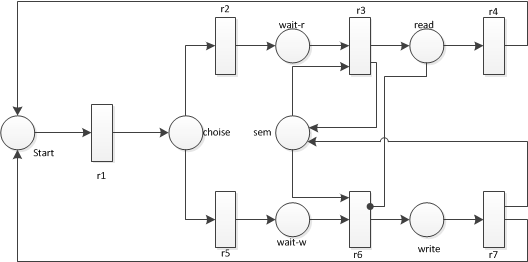
\includegraphics[width=10cm]{../resources/images/petri2.png}
	\label{petri2}
	\caption{Rete di petri simulata da CTMC-READER\_WRITER}
\end{figure}

Il modello si può esprimere in modo stocastico, facendo dipendere dal numero di
token i rate da un place all'altro. Implementativamente, per rapprentare gli
stati si utilizza un set di variabili, una per place, che hanno come valore il
numero di token.
\begin{Verbatim}[fontsize=\small]
var VL : VarList .
var N, M : Nat .

*** Start
crl [model] : < v("start" , N) v("choose" , M) VL > =>
             [10.0 * float(N)]
               < v("start" , N + -1) v("choose" , M + 1) VL >
             if N > 0 .
*** Read
crl [model] : < v("choose" , N) v("waitr" , M) VL > =>
             [5.0 * float(N)]
               < v("choose" , N + -1) v("waitr" , M + 1) VL >
             if N > 0 .
crl [model] : < v("waitr" , N) v("read" , M) v("sem" , 1) VL > =>
             [20.0 * float(N)]
               < v("waitr" , N + -1) v("read" , M + 1) v("sem" , 1) VL >
             if N > 0 .
crl [model] : < v("read" , N) v("start" , M) VL > =>
             [50.0 * float(N)]
               < v("read" , N + -1) v("start" , M + 1) VL >
             if N > 0 .
*** Write
crl [model] : < v("choose" , N) v("waitw" , M) VL > =>
             [5.0 * float(N)]
               < v("choose" , N + -1) v("waitw" , M + 1) VL >
             if N > 0 .
crl [model] : < v("waitw" , N) v("write" , M) v("sem" , 1)
                                            v("read" , 0) VL > =>
             [40.0 * float(N)]
               < v("waitw" , N + -1) v("write" , M + 1)
                                               v("sem" , 0) v("read" ,0) VL >
             
             if N > 0 .
crl [model] : < v("write" , N) v("start" , M) v("sem" , 0) VL > =>
             [50.0 * float(N)]
               < v("write" , N + -1) v("start" , M + 1) v("sem" , 1) VL >
             if N > 0 .

\end{Verbatim}

\subsubsection{Modello M/M/C/K per la simulazione delle code}
\label{sec:mmck}

M/M/C/K è un modello utilizzato nella teoria delle code per analizzare e
simulare il comportamento di un sistema di $C$ server che elaborano un task
alla volta. I task nascono con un certo rate $\tau$ e sono memorizzati in un
buffer di dimensione $K$. Se il buffer è pieno sono perduti. I task muoiono
(sono svolti dai server) con un rate che vale $\mu * N$, dove N è il numero dei
task, se $N \leq C$, altrimenti il rate vale $\mu * C$.

Gli stati del modello sono enumerabili da un numero naturale, tuttavia nel
modello sono inclusi anche altri elementi di configurazione ed utilità come la
dimensione del buffer, il numero di server e il numero di task perduti.

\begin{Verbatim}[fontsize=\small]
var N K L C : Nat .
var VL : VarList .

*** Accodamento nel Buffer
crl [model] : < v("buffersize" , K) v("buffer", N) VL > =>
              [ 0.535 ] < v("buffersize" , K) v("buffer", N + 1) VL >
              if N < K .
*** Buffer pieno
crl [model] : < v("buffersize" , K) v("buffer", N) v("losts", L) VL > =>
              [ 0.535 ] < v("buffersize" , K) v("buffer", N)
                                               v("losts", L + 1) VL >
              if N >= K .
*** Svolgimento di task (caso N < C)
crl [model] : < v("nserver" , C) v("buffer", N) VL > =>
              [0.120 * float(N)] < v("buffer", N + -1) v("nserver" , C) VL >
              if N > 0 /\ N < C .
*** Svolgimento di task (caso N >= C)
crl [model] : < v("nserver" , C) v("buffer", N) VL > =>
              [0.120 * float(C)] < v("buffer", N + -1) v("nserver" , C) VL >
              if N > 0 /\ N >= C .

\end{Verbatim}

\subsection{Modello di test della Bromosulftaleina}
\label{sec:bsf}

\begin{figure}[!ht]
	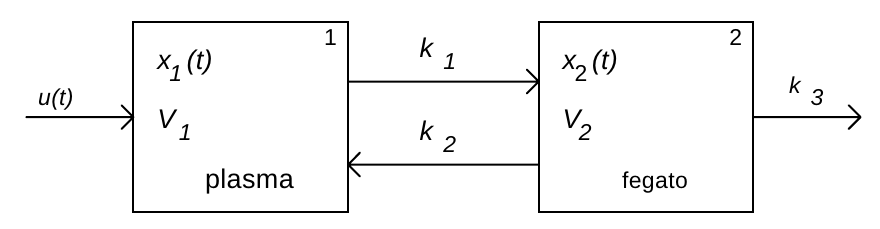
\includegraphics[width=10cm]{../resources/images/BSF.png}
	\label{bsf}
	\caption{Modello BSF (\cite{gnudi})}
\end{figure}

Il test BSF \cite{gnudi} è semplificabile considerandolo un sistema a due compartimenti
(uno per il fegato, l'altro per il plasma), con un certo rate di trasferimento. Si
suppone un inserimento del colorante nel plasma istantaneo e si può
semplificarlo imponendo la condizione inziale del plasma pari alla quantità di
colorante iniettato. Il colorante, quando entra nel fegato, scompare con un
certo rate e è riassorbito nel plasma con un altro rate. Per completezza si
considera anche il volume dei due compartimenti (vedi figura \ref{bsf}).

Il modello è semplificato al caso di trasferimenti di colorante discreti.

\begin{Verbatim}[fontsize=\small]
var N K L : Nat .
var VP VF : Nat .
var VL : VarList .
	
	
*** Passaggio colorante dal compartimento plasma a fegato
crl [model] : < v("volplasma", VP) v("volfegato", VF)
                       v("plasma", N) v("fegato", L) > =>
              [ 0.454 * float(N) / float(VP) ]
              < v("volplasma", VP) v("volfegato", VF)
                v("plasma", N + -1)  v("fegato", L + 1) >
              if N > 0 /\ L < VF .

*** Passaggio colorante dal compartimento fegato a plasma            
crl [model] : < v("volfegato", VF) v("volplasma", VP)
                       v("plasma", N) v("fegato", L) > =>
             [ 0.698 * float(L) / float(VF) ]
             < v("volfegato", VF) v("volplasma", VP)
               v("plasma", N + 1) v("fegato", L + -1) >
             if L > 0 /\ N < VP .
		
*** Scomparsa del colorante dal compartimento fegato
crl [model] : < v("volfegato", VF) v("fegato", L) VL > =>
             [ 0.432 * float(L) / float(VF) ]
             < v("volfegato", VF) v("fegato", L + -1) VL >
             if L > 0 .
	
\end{Verbatim}
\section{Approximate Probabilistic Model Checking}
\label{sec:APMC}
La PCTL (\emph{Probabilistic Computation Tree Logic}), permette di esprimere
proprietà che si avverano con una probabilità $\rho \in J$ su di un particolare
modello:
 \[
\phi ::= p | FALSE | \phi \rightarrow \phi' | P_J[\psi]
\]
\[
\psi ::= X \phi | \phi U \phi' | \phi U^I \phi'
\]

Dato un modello CTMC, la verifica di proprietà PCTL è un poblema
computazionalmente difficile a causa dell'esplosione degli stati da
verificare. Una prima semplificazione si può ottenere considerando solo
formule \emph{monotone}, in grado di ridurre lo spazio degli stati per
particolari proprietà. Una formula $\psi$ è monotona se e solo se \[\exists j
\in \mathbb{N}, \forall \pi{}[j..], \pi{}[j..]\models \phi \wedge \forall i \in
\mathbb{N}, i > j , \pi{}[i..]\models \phi \] 
Ovvero, una formula è monotona se la validità su di uno stato implica la
validità su tutte le path che partono da esso. Grazie a questa proprietà, la
verifica di $Prob_{\geq P}[ \psi ]$ può essere limitata alla verifica
$Prob_{\geq P}[ \psi ]_k$, ovvero limitata a path con profondità pari a $k$,
poiché la probabilità che la formula $\psi$ sia vera, può solo aumentare.
Formule composte unicamente da $FALSE$, proposizioni $p$, implicazioni $\phi
\rightarrow \phi{}'$ e operatori $X \phi$, $\phi U \phi{}'$ comprese le versioni bounded, sono formule monotone. Una grammatica per le formule monotone è la seguente:
 \[
\phi ::= p | FALSE | \phi \rightarrow \phi' | P_{\geq \rho}[\psi]
\]
\[
\psi ::= X \phi | \phi U \phi' | \phi U^I \phi'
\]

Le formule monotone non risolvono il problema della difficoltà
computazionale, ma rendono possibile applicare un procedimento approssimato,
ottenendo risultati appartenenti ad un intorno del vero risultato con una certa confidenza.

Il calcolo della probabilità si può approssimare con la tecnica di \emph{fully
polynomial randomized approximation scheme (FPRAS)} \cite{DBLP:conf/vmcai/2004}.
Un FPRAS è un algoritmo $A(x, \epsilon, \delta, k), \epsilon \in [0, 1], \delta
\in [0, 1]$ il quale, dato in input lo stato iniziale del sistema, una approssimazione, un parametro di confidenza e la lunghezza delle path
ritorna un valore di probabilità tale che:
\[
	Prob[ \mid A(x,\epsilon,\delta, k) - \mu(x) \mid \leq \epsilon] \geq 1 - \delta
\]
dove $\mu(x)$ è il risultato esatto della formula analizzata.

Una implementazione di $A$ è la seguente \cite{HLMP04}:

\vspace{0.3cm}
\fbox{%
        \parbox{0.7\linewidth}{%
A($x, \epsilon, \delta$) :\newline
$N := \log{\frac{2}{\delta}}/2\epsilon^2$\newline
$A := 0$\newline
for $i \in [1 ; N]$ do\newline
 1. Genera una path casuale $\pi$, di lunghezza $k$.\newline
 2. Se la formula $\phi$ da valutare è vera, $A := A + 1$.\newline 
$Return A/N$
      }%
}
\vspace{0.3cm}

L'algoritmo ha complessità polinomiale in $\frac{1}{\epsilon}$ e
$\log{\frac{1}{\delta}}$.

\section{Progetto PCTL}

La seconda parte del progetto riguarda l'implementazione di un verificatore di
proprietà PCTL utilizzando APMC.

\subsection{Strategia risolutiva}
\label{sec:strategia}
Il nuovo sistema, il verificatore, segue l'algoritmo descritto
nella sezione \ref{sec:APMC}. L'appossimazione $\epsilon$, il fattore di
confidenza $\delta$ e la profondità massima delle path sono forniti dall'utente
insieme allo stato iniziale, al modello e alla formula da verificare. 

Per la generazione della path casuale, sfrutto il simulatore CTMC
realizzato nella prima parte del progetto, ma anziché generare interamente una
path di profondità massima, simulo il sistema un passo alla volta, valutando la
formula in ogni nuovo stato.

In generale, per risolvere una formula seguo questo procedimento:
\begin{enumerate}
  \item Se la formula $f \in \phi$: risolvo la formula per lo
  stato corrente.
  \item Se la formula $f \in \psi , f = X \phi$: nello stato successivo
  verifico $\phi$.
  \item Se la formula $f \in \psi , f = \phi U \phi'$: se vale $\phi'$, $f$ è
  vera, altrimenti se vale $\phi$, nello stato successivo verifico $\phi U
  \phi'$. Se non vale né $\phi$ né $\phi'$, $f$ non è vera.
  \item Se la formula $f \in \psi , f = \phi U^{\leq\tau} \phi'$: se vale
  $\phi'$, $f$ è vera, alrimenti se vale $\phi$, nello stato successivo verifico
  $\phi U^{\leq\tau} \phi$. Se non vale né $\phi$ né $\phi'$, $f$ non è vera. Se
  arrivo in uno stato in cui il tempo $t > \tau$, la formula $f$ non è vera.
\end{enumerate}


\subsection{Sintassi delle Formule}
All'interno del modulo \emph{PCTL}, ho definito i sort e i costruttori necessari
a definire le formule PCTL. Come predicato $p$, utilizzo meta-stato \emph{Term},
con semantica $p \equiv S$, dove $S$ è il meta-stato corrente, oppure
$p(State, Condition)$ in grado di definire predicati contenenti stati che
effettuano un match con lo stato corrente e che devono rispettare certe
condizioni con sintassi definita dal sort \emph{Condition} \cite{maudemanual}.

\begin{Verbatim}[fontsize=\small]
*** Formula -> phi ; PathFormula -> psi
sort Formula PathFormula .

*** Un predicato p è un meta-stato.
subsort Term < Formula .
*** p(Term, Condition) effettua un matching di Term con lo stato corrente,
*** controllando la Condition.
op p : Term Condition -> Formula [ ctor ] .
op FALSE : -> Formula [ ctor ] .
op TRUE : -> Formula [ ctor ] .
op _ implies _ : Formula Formula -> Formula [ ctor prec 90 ] .
op _ and _ : Formula Formula -> Formula [ ctor prec 80 ] .
op _ or _ : Formula Formula -> Formula [ ctor prec 80 ] .
op not _ : Formula -> Formula [ ctor prec 75 ] .
op P[_](_) : Float PathFormula -> Formula [ ctor prec 70] .

op (_)U[_](_) : Formula Float Formula -> PathFormula [ ctor prec 92] .
op (_)U(_) : Formula Formula -> PathFormula [ ctor prec 92] .
op X_ : Formula -> PathFormula [ ctor ] .
*** Per risolvere ricorsivamente X phi, creo un altro operatore C phi:
*** true se phi vale nello stato corrente
op C_ : Formula -> PathFormula [ ctor ] .
\end{Verbatim}

Il costruttore \emph{C\_} è un artefatto che ho introdotto per semplificare la
risoluzione ricorsiva delle \emph{PathFormula} ($\psi$). Il significato
semantico di $C\phi$ è ``nello stato corrente deve valere $\phi$''.
L'operatore \emph{P[\_](\_)} rappresenta l'operatore di probabilità e il suo
significato è : $Prob_{\geq p}(\psi)$.

L'operatore $p(S1, C)$ è verificato se , con stato corrente $S$, esiste un
matching fra $S1$ e $S$ che rispetti la condizione $C$. Questa procedura è
facilmente implementabile attraverso la \emph{metaXmatch} imponendo che il
Context sia vuoto, ovvero che non esistano termini senza matching.

 \begin{Verbatim}[fontsize=\small]
***
*** match(M, t1, t2, tc) verifica che esista un matching fra il meta-stato.
*** t1 e l'intero meta-stato t2, rispettando la condizione tc.
***   - Module : meta-modulo utente.
***   - Term : meta-stato da verificare.
***   - Term : meta-stato corrente.
***   - Condition : condizione che il meta-stato da verificare deve rispettare.
op match : Module Term Term Condition -> Bool .
\end{Verbatim}

\subsection{Verifica di Proprietà}

Per verificare una formula su un modello a partire da un certo stato
iniziale, si utilizza l'operazione \emph{verify}, specificando il nome del
modulo utente, il meta-stato iniziale, la formula e tutti i parametri necessari.
L'operazione \emph{verify} funge da wrapper per una operazione \emph{verify}
con differenti argomenti, che verifica la formula.

\begin{Verbatim}[fontsize=\small]
***
*** Verfica la formula data (entry point)
***   - Qid : Nome del modulo utente su cui c'è il modello .
***   - Formula : formula PCTL fa verificare.
***   - Term : meta-stato iniziale
***   - Float : approximation.
***   - Float : Confidence.
***   - Nat : Max Depth.
***   - Nat : indice di partenza per la generazione di numeri casuali.
op verify : Qid Formula Term Float Float Nat Nat -> Bool .
	
***
*** Verfica la formula data
***   - Module : meta-modulo utente.
***   - Formula : formula PCTL fa verificare.
***   - SimulationResult : meta-stato corrente + tempo + deadlock?
***   - Float : approximation.
***   - Float : Confidence.
***   - Nat : Max Depth.
***   - Nat : indice di partenza per la generazione di numeri casuali.
op verify : Module Formula SimulationResult Float Float Nat Nat -> Bool .
\end{Verbatim}

L'operazione verify, verifica le formule $\phi$. Quando compare una formula del
tipo \emph{P[\_]($\psi$)}, è computato il numero di sample $N$ da
effettuare e verify richiama l'operazione \emph{approxChecking} che per $N$ volte crea una
path random verificando la formula $\psi$. Come ulteriore miglioramento delle
prestazioni, interrompo il model checking se la probabilità incrementale ha già
raggiunto la probabilità target (le formule sono monotone, dunque la
probabilità può solo aumentare ulteriormente).
	
\begin{Verbatim}[fontsize=\small]
***
*** Esegue un model checking approssimato della PathFormula data
***   - Module : meta-modulo utente. 
***   - PathFormula : path-formula PCTL fa verificare.
***   - SimulationResult : Stato corrente + tempo.
***   - Nat : Numero di campioni corretti.
***   - Nat : Numero di campioni testati.
***   - Nat : Numero di campioni massimi.
***   - Float : Probabilità da raggiungere.
***   - Float : approximation.
***   - Float : Confidence.
***   - Nat : Max Depth.
***   - Nat : indice di partenza per la generazione di numeri casuali. 
op approxChecking : Module PathFormula SimulationResult
                    Nat Nat Nat Float Float Float Nat Nat -> Float  .
\end{Verbatim}

Per verificare una formula all'interno durante la generazione di una path, ho
creato una operazione \emph{checkOnRandomPath} che ricorsivamente incrementa di
un passo la simulazione, verificando di volta in volta $\psi$, seguendo le
strategie descritte nella sezione \ref{sec:strategia}:
\begin{description}
  \item[$\phi_1 U \phi_2$:]nello stato corrente verifico $\phi_2$,
  se è vera, allora la formula è verificata, altrimenti verifico $\phi_1$. Se
  $\phi_1$ è false, allora la formula è falsa, altrimenti avanzo la simulazione
  di un passo con l'operazione \emph{simNcheck}, verificando nello stato
  successivo la stessa formula $\phi_1 U \phi_2$.
  \item[$\phi_1 U^{\leq \tau} \phi_2$:] si comporta esattamente come la versione
  non bounded, ma prima di tutto controllo se $\tau \geq t$, dove $t$ è il tempo
  nello stato corrente. Se la relazione è falsa, la formula non è verificata.
  \item[$X \phi$:]avanzo la simulazione di un passo con l'operazione
  \emph{simNcheck}, verificando nello stato successivo la formula $C \phi$.
  \item[$C \phi$:]controllo nello stato corrente se $\phi$ è verificata.
\end{description}

Ovviamente la verifica di $\phi$ avviene richiamando l'operazione \emph{verify}.
\begin{Verbatim}[fontsize=\small]
***
*** Controlla una PathFormula su una path casuale
***   - Module : meta-modulo utente.
***   - PathFormula : path-formula PCTL da verificare.
***   - SimulationResult : Stato corrente + tempo.
***   - Nat : Profondità corrente.
***   - Nat : Profondità massima.
***   - Float : approximation.
***   - Float : Confidence.
***   - Nat : indice di partenza per la generazione di numeri casuali.
op checkOnRandomPath : Module PathFormula SimulationResult
                             Nat Nat Float Float Nat -> Bool .
                             
***
*** Esegue una simulazione di un passo e controlla la PathFormula
*** sul nuovo stato.
***   - Module : meta-modulo utente
***   - PathFormula : path-formula PCTL da verificare nello
***                                              stato successivo.
***   - SimulationResult : Stato corrente + tempo
***   - Nat : Profondità corrente
***   - Nat : Profondità massima
***   - Float : approximation
***   - Float : Confidence
***   - Nat : indice di partenza per la generazione di numeri casuali
op simNcheck : Module PathFormula SimulationResult
                              Nat Nat Float Float Nat -> Bool .

\end{Verbatim}

\subsection{Confronto con PRISM}

Se con il framework realizzato si può avere una maggiore espressività
rispetto a PRISM, lo si paga enormemente nelle prestazioni. Di seguito riporto
dei test che ho effettuato su tre moduli diversi, descritti nella sezione
\ref{sec:esempio}. PRISM mette a disposizione l'operatore $P=?[ \ldots ]$, che
ritorna la probabilità anziché un booleano. Per ottenere lo stesso risultato nel
framework, basta valutare $P[1.0]( \ldots )$ e abilitare le print con il comando
\begin{Verbatim}
Maude> set print attribute on .
\end{Verbatim}
Al termine della valutazione è stampato il valore di probabilità finale.

\subsubsection{Modello readers-writers}

Il modello readers-writers è descritto nella sezione \ref{sec:rw}. Di seguito
riporto anche la sua implementazione in PRISM:
\begin{Verbatim}[fontsize=\small]
ctmc

// Numero di processi
const int N = 100;

module RW
start : [0..N] init N;
choise : [0..N] init 0;
waitr : [0..N] init 0;
waitw : [0..N] init 0;
sem : [0..N] init 1;
read : [0..N] init 0;
write : [0..N] init 0;

[t1] start>0 & choise<N  -> start :
     (start'=start-1)&(choise'=choise+1);
[t2] choise>0 & waitr<N & waitw<N -> choise :
     (choise'=choise-1) & (waitr'=waitr+1);
[t3] choise>0 & waitr<N & waitw<N -> choise :
     (choise'=choise-1) & (waitw'=waitw+1);
[t4] waitr>0 & sem>0 & read<N -> waitr*sem :
     (waitr'=waitr-1) & (read'=read+1);
[t5] waitw>0 & sem>0 & read=0 & write<N -> waitw*sem :
     (waitw'=waitw-1) & (sem'=sem-1) & (write'=write+1);
[t6] read>0 & start<N -> read :
     (read'=read-1) & (start'=start+1);
[t7] write>0 & sem<N & start<N -> write :
     (write'=write-1) & (start'=start+1) & (sem'=sem+1);

endmodule

// Definizione dei rate

const double r1=10;
const double r2=5;
const double r3=5;
const double r4=20;
const double r5=40;
const double r6=50;
const double r7=50;

module base_rate 
[t1] true  -> r1 : true;
[t2] true  -> r2 : true;
[t3] true  -> r3 : true;
[t4] true  -> r4 : true;
[t5] true  -> r5 : true;
[t6] true  -> r6 : true;
[t7] true  -> r7 : true;
endmodule
\end{Verbatim}

Il test è stato fatto con condizione iniziale 100 processi, 10000 profondità
massima, $\epsilon = 0.01$ e $\delta = 1.0\cdot10^{-10}$.

\textbf{P=?[true U[0.1] waitw $>$ 0 $\&$ read $>$ 0]} (la probabilità che entro
0.1 secondi, ci sia un processo in lettura ed uno in attesa di scrivere).
La formula espressa nel framework è:
\begin{Verbatim}
red in CTMC-RW_VERIFIER : verify(100,
 P[1.0] ( (TRUE) U[0.1] ( 
    p( upTerm(< v("read", N:Nat) v("waitw", M:Nat) V:VarList >),
                  upTerm(N:Nat > 0 and M:Nat > 0) = 'true.Bool )))
   , 0.01, 0.0000000001, 10000, 42793) .
\end{Verbatim}
Dove CTMC-RW\_VERIFIER è un wrapper per facilitare la verifica delle operazioni
di verifica sul modulo CTMC-READER\_WRITER.

\begin{description}
	\item[PRISM:] tempo: 17.855 secondi . Probabilità: 0.7882288460727687
	\item[ENGINE:] tempo: 2036.773 secondi . Probabilità: 0.77615413803280076
\end{description}

La differenza di probabilità è 0.012074708, quindi rientra nei limiti
dell'approssimazione.

\subsubsection{Modello BSF}

Il modello del test della Bromosulftaleina è descritto nella sezione
\ref{sec:bsf}. Di seguito riporto anche la sua implementazione in PRISM:
\begin{Verbatim}[fontsize=\small]
ctmc
// Volume Plasma
const int VP = 1000;
// Volume Fegato
const int VF = 800;
// Colorante iniziale
const int IC = 500;

module BSF
Pl : [0..VP] init IC;
Fe : [0..VF] init 0;

[t1] Pl > 0 & Fe < VF -> Pl / VP :
      (Pl'=Pl-1) & (Fe'=Fe+1);
[t2] Fe > 0 & Pl < VP -> Fe / VF :
     (Pl'=Pl+1) & (Fe'=Fe-1);
[t3] Fe > 0 -> Fe / VF :
     (Fe'=Fe-1);

endmodule

//base rates

const double r1=0.454;
const double r2=0.698;
const double r3=0.432;

module base_rate 
[t1] true  -> r1 : true;
[t2] true  -> r2 : true;
[t3] true  -> r3 : true;
endmodule
\end{Verbatim}


Il test è stato fatto con condizione iniziale 800 volume fegato, 1000 volume
plasma, 500 colorante, 10000 profondità massima , $\epsilon = 0.05$ e
$\delta = 1.0\cdot10^{-4}$. \textbf{P=?[true U[50000] Fe = 0 $\&$ Pl = 0]}.
La formula espressa nel framework è:
\begin{Verbatim}
red in CTMC-BSF_VERIFIER : verify(1000, 800, 500,
 P[1.0] ( (TRUE) U[50000.0] ( 
    upTerm(< v("plasma", 0) v("fegato", 0) V:VarList >)))
   , 0.05, 0.0001, 10000, 1351) .
\end{Verbatim}
Dove CTMC-BSF\_VERIFIER è un wrapper per facilitare la verifica delle operazioni
di verifica sul modulo CTMC-BSF.

\begin{description}
	\item[PRISM:] tempo: 6.874 secondi . Probabilità: 0.6431095406360424
	\item[ENGINE:] tempo: 984.625 secondi . Probabilità: 0.69863705199394244
\end{description}

La differenza di probabilità è 0.055527511, quindi rientra nei limiti
dell'approssimazione.

\subsubsection{Modello MMCK}

Il modello del test M/M/C/K è descritto nella sezione
\ref{sec:mmck}. Di seguito riporto anche la sua implementazione in PRISM:
\begin{Verbatim}[fontsize=\small]
ctmc
// Numero di server (C)
const int nServ = 5;
// Dimension del buffer (K)
const int buffSize = 10;

const int lostSize = 1000;

module MMCK
Buff : [0..buffSize] init 0;
Losts : [0..lostSize] init 0;

[t1] Buff < buffSize ->
     (Buff'=Buff+1);
[t2] Buff >= buffSize & Losts < lostSize ->
     (Losts'=Losts+1);
[t3] Buff > 0 & Buff < nServ -> Buff :
     (Buff'=Buff-1);
[t4] Buff >= nServ -> nServ : 
     (Buff'=Buff-1);

endmodule

//base rates

const double r1=0.535;
const double r2=0.120;

module base_rate 
[t1] true  -> r1 : true;
[t2] true  -> r1 : true;
[t3] true  -> r2 : true;
[t4] true  -> r2 : true;
endmodule
\end{Verbatim}

Il test è stato fatto con condizione iniziale 10 dimensione buffer, 5 server,
profondità massima $K = 10000$, $\epsilon = 0.01$ e $\delta = 1.0\cdot10^{-10}$.

\textbf{P=?[true U[70.0] losts $>$ 0]} (la probabilità che il buffer regga
almeno 50 secondi). La formula espressa nel framework è:
\begin{Verbatim}
red in CTMC-MMCK_VERIFIER : verify(10, 5,
 P[1.0] ( (TRUE) U[70.0] ( 
    upTerm(< v("losts", 1) V:VarList >)))
   , 0.01, 0.0000000001, 10000, 12523) .
\end{Verbatim}
Dove CTMC-MMCK\_VERIFIER è un wrapper per facilitare la verifica delle
operazioni di verifica sul modulo CTMC-MMCK.

\begin{description}
	\item[PRISM:] tempo: 6.689 secondi . Probabilità: 0.41349972595809265
	\item[ENGINE:] tempo: 1227.478 secondi . Probabilità: 0.40806948016358197
\end{description}

La differenza di probabilità è  0.005430246, quindi rientra nei limiti
dell'approssimazione.


\bibliographystyle{plain}
\bibliography{bib/bib}

\end{document}